\documentclass[NEMO_book]{subfiles}
\begin{document}
% ================================================================
% Chapter � Miscellaneous Topics
% ================================================================
\chapter{Miscellaneous Topics}
\label{MISC}
\minitoc

\newpage
$\ $\newline    % force a new ligne

% ================================================================
% Representation of Unresolved Straits
% ================================================================
\section{Representation of Unresolved Straits}
\label{MISC_strait}

In climate modeling, it often occurs that a crucial connections between water masses
is broken as the grid mesh is too coarse to resolve narrow straits. For example, coarse 
grid spacing typically closes off the Mediterranean from the Atlantic at the Strait of 
Gibraltar. In this case, it is important for climate models to include the effects of salty 
water entering the Atlantic from the Mediterranean. Likewise, it is important for the 
Mediterranean to replenish its supply of water from the Atlantic to balance the net 
evaporation occurring over the Mediterranean region. This problem occurs even in 
eddy permitting simulations. For example, in ORCA 1/4\deg several straits of the Indonesian 
archipelago (Ombai, Lombok...) are much narrow than even a single ocean grid-point.

We describe briefly here the three methods that can be used in \NEMO to handle 
such improperly resolved straits. The first two consist of opening the strait by hand 
while ensuring that the mass exchanges through the strait are not too large by 
either artificially reducing the surface of the strait grid-cells or, locally increasing 
the lateral friction. In the third one, the strait is closed but exchanges of mass, 
heat and salt across the land are allowed.
Note that such modifications are so specific to a given configuration that no attempt 
has been made to set them in a generic way. However, examples of how 
they can be set up is given in the ORCA 2\deg and 0.5\deg configurations. For example, 
for details of implementation in ORCA2, search: 
\texttt{ IF( cp\_cfg == "orca" .AND. jp\_cfg == 2 ) }

% -------------------------------------------------------------------------------------------------------------
%       Hand made geometry changes
% -------------------------------------------------------------------------------------------------------------
\subsection{Hand made geometry changes}
\label{MISC_strait_hand}

$\bullet$ reduced scale factor in the cross-strait direction to a value in better agreement 
with the true mean width of the strait. (Fig.~\ref{Fig_MISC_strait_hand}).
This technique is sometime called "partially open face" or "partially closed cells".
The key issue here is only to reduce the faces of $T$-cell ($i.e.$ change the value 
of the horizontal scale factors at $u$- or $v$-point) but not the volume of the $T$-cell.
Indeed, reducing the volume of strait $T$-cell can easily produce a numerical 
instability at that grid point that would require a reduction of the model time step.
The changes associated with strait management are done in \mdl{domhgr}, 
just after the definition or reading of the horizontal scale factors. 

$\bullet$ increase of the viscous boundary layer thickness by local increase of the 
fmask value at the coast (Fig.~\ref{Fig_MISC_strait_hand}). This is done in 
\mdl{dommsk} together with the setting of the coastal value of fmask 
(see Section \ref{LBC_coast})

%>>>>>>>>>>>>>>>>>>>>>>>>>>>>
\begin{figure}[!tbp] 	 \begin{center}
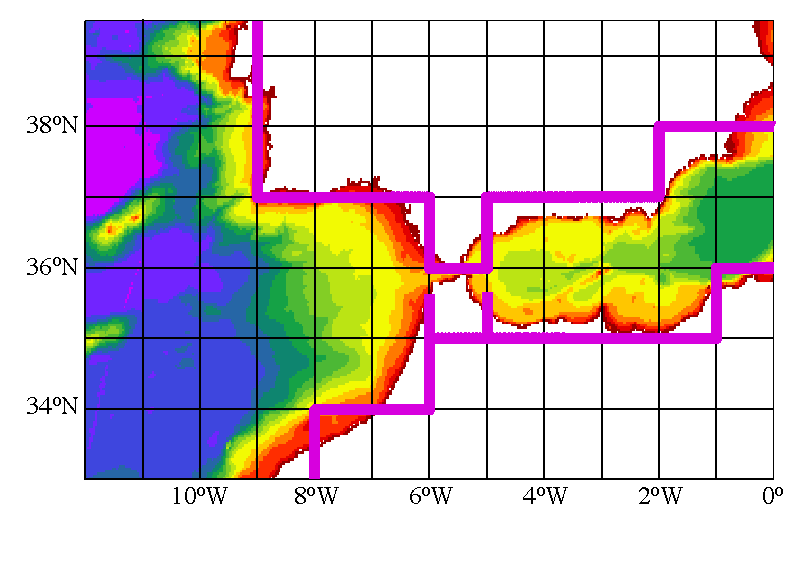
\includegraphics[width=0.80\textwidth]{Fig_Gibraltar}
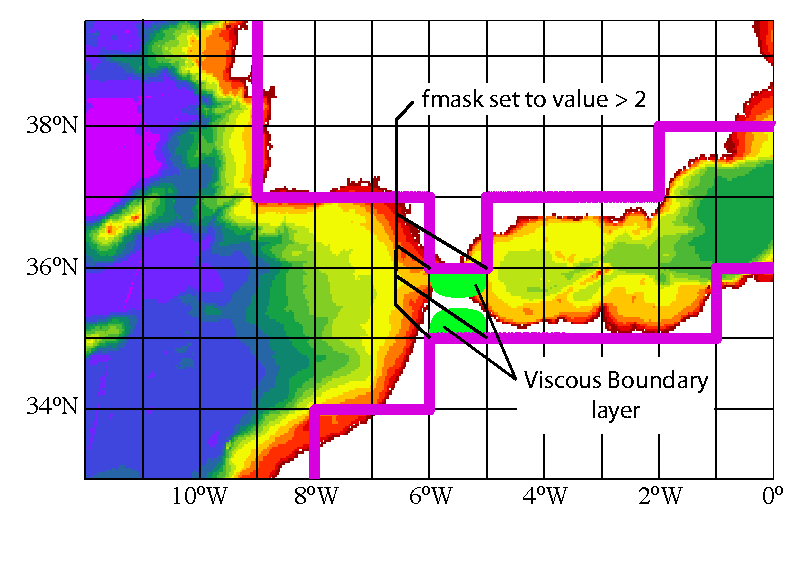
\includegraphics[width=0.80\textwidth]{Fig_Gibraltar2}
\caption{	\label{Fig_MISC_strait_hand} 
Example of the Gibraltar strait defined in a $1^{\circ} \times 1^{\circ}$ mesh. 
\textit{Top}: using partially open cells. The meridional scale factor at $v$-point 
is reduced on both sides of the strait to account for the real width of the strait 
(about 20 km). Note that the scale factors of the strait $T$-point remains unchanged. 
\textit{Bottom}: using viscous boundary layers. The four fmask parameters 
along the strait coastlines are set to a value larger than 4, $i.e.$ "strong" no-slip 
case (see Fig.\ref{Fig_LBC_shlat}) creating a large viscous boundary layer 
that allows a reduced transport through the strait.}
\end{center}   \end{figure}
%>>>>>>>>>>>>>>>>>>>>>>>>>>>>

% -------------------------------------------------------------------------------------------------------------
% Cross Land Advection 
% -------------------------------------------------------------------------------------------------------------
\subsection{Cross Land Advection (\mdl{tracla})}
\label{MISC_strait_cla}
%--------------------------------------------namcla--------------------------------------------------------
\namdisplay{namcla} 
%--------------------------------------------------------------------------------------------------------------

Options are defined through the  \ngn{namcla} namelist variables.
This option is an obsolescent feature that will be removed in version 3.7 and followings. 

%The problem is resolved here by allowing the mixing of tracers and mass/volume between non-adjacent water columns at nominated regions within the model. Momentum is not mixed. The scheme conserves total tracer content, and total volume (the latter in $z*$- or $s*$-coordinate), and maintains compatibility between the tracer and mass/volume budgets.  

% ================================================================
% Closed seas
% ================================================================
\section{Closed seas (\mdl{closea})}
\label{MISC_closea}

\colorbox{yellow}{Add here a short description of the way closed seas are managed}


% ================================================================
% Sub-Domain Functionality (\textit{nizoom, njzoom}, namelist parameters)
% ================================================================
\section{Sub-Domain Functionality (\np{jpizoom}, \np{jpjzoom})}
\label{MISC_zoom}

The sub-domain functionality, also improperly called the zoom option 
(improperly because it is not associated with a change in model resolution) 
is a quite simple function that allows a simulation over a sub-domain of an 
already defined configuration ($i.e.$ without defining a new mesh, initial 
state and forcings). This option can be useful for testing the user settings 
of surface boundary conditions, or the initial ocean state of a huge ocean 
model configuration while having a small computer memory requirement. 
It can also be used to easily test specific physics in a sub-domain (for example, 
see \citep{Madec_al_JPO96} for a test of the coupling used in the global ocean 
version of OPA between sea-ice and ocean model over the Arctic or Antarctic 
ocean, using a sub-domain). In the standard model, this option does not 
include any specific treatment for the ocean boundaries of the sub-domain: 
they are considered as artificial vertical walls. Nevertheless, it is quite easy 
to add a restoring term toward a climatology in the vicinity of such boundaries 
(see \S\ref{TRA_dmp}).

In order to easily define a sub-domain over which the computation can be 
performed, the dimension of all input arrays (ocean mesh, bathymetry, 
forcing, initial state, ...) are defined as \np{jpidta}, \np{jpjdta} and \np{jpkdta} 
( in \ngn{namcfg} namelist), while the computational domain is defined through 
\np{jpiglo}, \np{jpjglo} and \jp{jpk} (\ngn{namcfg} namelist). When running the 
model over the whole domain, the user sets \np{jpiglo}=\np{jpidta} \np{jpjglo}=\np{jpjdta} 
and \jp{jpk}=\jp{jpkdta}. When running the model over a sub-domain, the user 
has to provide the size of the sub-domain, (\np{jpiglo}, \np{jpjglo}, \np{jpkglo}), 
and the indices of the south western corner as \np{jpizoom} and \np{jpjzoom} in 
the  \ngn{namcfg} namelist (Fig.~\ref{Fig_LBC_zoom}). 

Note that a third set of dimensions exist, \jp{jpi}, \jp{jpj} and \jp{jpk} which is 
actually used to perform the computation. It is set by default to \jp{jpi}=\np{jpjglo} 
and \jp{jpj}=\np{jpjglo}, except for massively parallel computing where the 
computational domain is laid out on local processor memories following a 2D 
horizontal splitting. % (see {\S}IV.2-c) ref to the section to be updated

\subsection{Simple subsetting of input files via netCDF attributes}

The extended grids for use with the under-shelf ice cavities will result in redundant rows
around Antarctica if the ice cavities are not active. A simple mechanism for subsetting
input files associated with the extended domains has been implemented to avoid the need to
maintain different sets of input fields for use with or without active ice cavities. The
existing 'zoom' options are overly complex for this task and marked for deletion anyway.
This alternative subsetting operates for the j-direction only and works by optionally
looking for and using a global file attribute (named: \np{open\_ocean\_jstart}) to
determine the starting j-row for input. The use of this option is best explained with an
example: Consider an ORCA1 configuration using the extended grid bathymetry and coordinate
files:
\vspace{-10pt}
\begin{alltt}
\tiny
\begin{verbatim}
eORCA1_bathymetry_v2.nc
eORCA1_coordinates.nc
\end{verbatim}
\end{alltt}
\noindent These files define a horizontal domain of 362x332. Assuming the first row with
open ocean wet points in the non-isf bathymetry for this set is row 42 (Fortran indexing)
then the formally correct setting for \np{open\_ocean\_jstart} is 41. Using this value as the
first row to be read will result in a 362x292 domain which is the same size as the original
ORCA1 domain. Thus the extended coordinates and bathymetry files can be used with all the
original input files for ORCA1 if the ice cavities are not active (\np{ln\_isfcav =
.false.}). Full instructions for achieving this are:

\noindent Add the new attribute to any input files requiring a j-row offset, i.e:
\vspace{-10pt}
\begin{alltt}
\tiny
\begin{verbatim}
ncatted  -a open_ocean_jstart,global,a,d,41 eORCA1_coordinates.nc 
ncatted  -a open_ocean_jstart,global,a,d,41 eORCA1_bathymetry_v2.nc
\end{verbatim}
\end{alltt}
 
\noindent Add the logical switch to \ngn{namcfg} in the configuration namelist and set true:
%--------------------------------------------namcfg--------------------------------------------------------
\namdisplay{namcfg_orca1}
%--------------------------------------------------------------------------------------------------------------

\noindent Note the j-size of the global domain is the (extended j-size minus
\np{open\_ocean\_jstart} + 1 ) and this must match the size of all datasets other than
bathymetry and coordinates currently. However the option can be extended to any global, 2D
and 3D, netcdf, input field by adding the:
\vspace{-10pt}
\begin{alltt}
\tiny
\begin{verbatim}
lrowattr=ln_use_jattr
\end{verbatim}
\end{alltt}
optional argument to the appropriate \np{iom\_get} call and the \np{open\_ocean\_jstart} attribute to the corresponding input files. It remains the users responsibility to set \np{jpjdta} and \np{jpjglo} values in the \np{namelist\_cfg} file according to their needs.

%>>>>>>>>>>>>>>>>>>>>>>>>>>>>
\begin{figure}[!ht] 	  \begin{center}
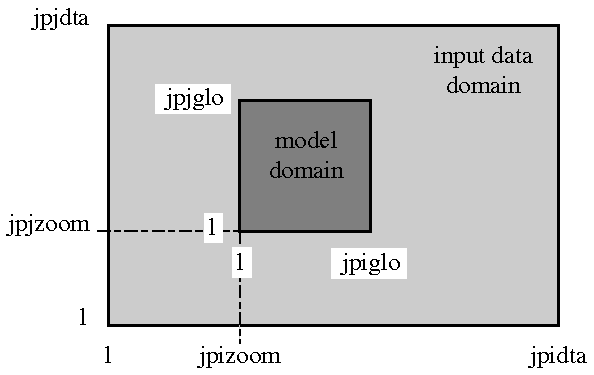
\includegraphics[width=0.90\textwidth]{Fig_LBC_zoom}
\caption{	\label{Fig_LBC_zoom}
Position of a model domain compared to the data input domain when the zoom functionality is used.}
\end{center}   \end{figure}
%>>>>>>>>>>>>>>>>>>>>>>>>>>>>


% ================================================================
% Accelerating the Convergence 
% ================================================================
\section{Accelerating the Convergence (\np{nn\_acc} = 1)}
\label{MISC_acc}
%--------------------------------------------namdom-------------------------------------------------------
\namdisplay{namdom} 
%--------------------------------------------------------------------------------------------------------------

Searching an equilibrium state with an global ocean model requires a very long time 
integration period (a few thousand years for a global model). Due to the size of 
the time step required for numerical stability (less than a few hours), 
this usually requires a large elapsed time. In order to overcome this problem, 
\citet{Bryan1984} introduces a technique that is intended to accelerate 
the spin up to equilibrium. It uses a larger time step in 
the tracer evolution equations than in the momentum evolution 
equations. It does not affect the equilibrium solution but modifies the 
trajectory to reach it.

Options are defined through the  \ngn{namdom} namelist variables.
The acceleration of convergence option is used when \np{nn\_acc}=1. In that case, 
$\rdt=rn\_rdt$ is the time step of dynamics while $\widetilde{\rdt}=rdttra$ is the 
tracer time-step. the former is set from the \np{rn\_rdt} namelist parameter while the latter
is computed using a hyperbolic tangent profile and the following namelist parameters : 
\np{rn\_rdtmin}, \np{rn\_rdtmax} and \np{rn\_rdth}. Those three parameters correspond 
to the surface value the deep ocean value and the depth at which the transition occurs, respectively. 
The set of prognostic equations to solve becomes:
\begin{equation} \label{Eq_acc}
\begin{split}
\frac{\partial \textbf{U}_h }{\partial t} 
	&\equiv \frac{\textbf{U}_h ^{t+1}-\textbf{U}_h^{t-1} }{2\rdt} = \ldots \\ 
\frac{\partial T}{\partial t} &\equiv \frac{T^{t+1}-T^{t-1}}{2 \widetilde{\rdt}} = \ldots \\ 
\frac{\partial S}{\partial t} &\equiv \frac{S^{t+1} -S^{t-1}}{2 \widetilde{\rdt}} = \ldots \\ 
\end{split}
\end{equation}

\citet{Bryan1984} has examined the consequences of this distorted physics. 
Free waves have a slower phase speed, their meridional structure is slightly 
modified, and the growth rate of baroclinically unstable waves is reduced 
but with a wider range of instability. This technique is efficient for 
searching for an equilibrium state in coarse resolution models. However its 
application is not suitable for many oceanic problems: it cannot be used for 
transient or time evolving problems (in particular, it is very questionable 
to use this technique when there is a seasonal cycle in the forcing fields), 
and it cannot be used in high-resolution models where baroclinically 
unstable processes are important. Moreover, the vertical variation of 
$\widetilde{ \rdt}$ implies that the heat and salt contents are no longer 
conserved due to the vertical coupling of the ocean level through both 
advection and diffusion. Therefore \np{rn\_rdtmin} = \np{rn\_rdtmax} should be
a more clever choice.


% ================================================================
% Accuracy and Reproducibility
% ================================================================
\section{Accuracy and Reproducibility (\mdl{lib\_fortran})}
\label{MISC_fortran}

\subsection{Issues with intrinsinc SIGN function (\key{nosignedzero})}
\label{MISC_sign}

The SIGN(A, B) is the \textsc {Fortran} intrinsic function delivers the magnitude 
of A with the sign of B. For example, SIGN(-3.0,2.0) has the value 3.0.
The problematic case is when the second argument is zero, because, on platforms 
that support IEEE arithmetic, zero is actually a signed number. 
There is a positive zero and a negative zero.

In \textsc{Fortran}~90, the processor was required always to deliver a positive result for SIGN(A, B) 
if B was zero. Nevertheless, in \textsc{Fortran}~95, the processor is allowed to do the correct thing 
and deliver ABS(A) when B is a positive zero and -ABS(A) when B is a negative zero. 
This change in the specification becomes apparent only when B is of type real, and is zero, 
and the processor is capable of distinguishing between positive and negative zero, 
and B is negative real zero. Then SIGN delivers a negative result where, under \textsc{Fortran}~90 
rules,  it used to return a positive result. 
This change may be especially sensitive for the ice model, so we overwrite the intrinsinc 
function with our own function simply performing :   \\
\verb?   IF( B >= 0.e0 ) THEN   ;   SIGN(A,B) = ABS(A)  ?    \\
\verb?   ELSE                   ;   SIGN(A,B) =-ABS(A)     ?  \\
\verb?   ENDIF    ? \\
This feature can be found in \mdl{lib\_fortran} module and is effective when \key{nosignedzero}
is defined. We use a CPP key as the overwritting of a intrinsic function can present 
performance issues with some computers/compilers.


\subsection{MPP reproducibility}
\label{MISC_glosum}

The numerical reproducibility of simulations on distributed memory parallel computers 
is a critical issue. In particular, within NEMO global summation of distributed arrays 
is most susceptible to rounding errors, and their propagation and accumulation cause 
uncertainty in final simulation reproducibility on different numbers of processors.
To avoid so, based on \citet{He_Ding_JSC01} review of different technics, 
we use a so called self-compensated summation method. The idea is to estimate 
the roundoff error, store it in a buffer, and then add it back in the next addition. 

Suppose we need to calculate $b = a_1 + a_2 + a_3$. The following algorithm 
will allow to split the sum in two ($sum_1 = a_{1} + a_{2}$ and $b = sum_2 = sum_1 + a_3$) 
with exactly the same rounding errors as the sum performed all at once.
\begin{align*}
	sum_1 \ \  &= a_1 + a_2 \\
	error_1     &= a_2 + ( a_1 - sum_1 ) \\
	sum_2 \ \  &= sum_1 + a_3 + error_1 \\
	error_2     &= a_3 + error_1 + ( sum_1 - sum_2 ) \\
	b \qquad \ &= sum_2 \\
\end{align*}
This feature can be found in \mdl{lib\_fortran} module and is effective when \key{mpp\_rep}.
In that case, all calls to glob\_sum function (summation over the entire basin excluding 
duplicated rows and columns due to cyclic or north fold boundary condition as well as 
overlap MPP areas). 
Note this implementation may be sensitive to the optimization level. 

\subsection{MPP scalability}
\label{MISC_mppsca}

The default method of communicating values across the north-fold in distributed memory applications
(\key{mpp\_mpi}) uses a \textsc{MPI\_ALLGATHER} function to exchange values from each processing
region in the northern row with every other processing region in the northern row. This enables a
global width array containing the top 4 rows to be collated on every northern row processor and then
folded with a simple algorithm. Although conceptually simple, this "All to All" communication will
hamper performance scalability for large numbers of northern row processors. From version 3.4
onwards an alternative method is available which only performs direct "Peer to Peer" communications
between each processor and its immediate "neighbours" across the fold line. This is achieved by
using the default \textsc{MPI\_ALLGATHER} method during initialisation to help identify the "active"
neighbours. Stored lists of these neighbours are then used in all subsequent north-fold exchanges to
restrict exchanges to those between associated regions. The collated global width array for each
region is thus only partially filled but is guaranteed to be set at all the locations actually
required by each individual for the fold operation. This alternative method should give identical
results to the default \textsc{ALLGATHER} method and is recommended for large values of \np{jpni}.
The new method is activated by setting \np{ln\_nnogather} to be true ({\bf nammpp}). The
reproducibility of results using the two methods should be confirmed for each new, non-reference
configuration.

% ================================================================
% Model optimisation, Control Print and Benchmark
% ================================================================
\section{Model Optimisation, Control Print and Benchmark}
\label{MISC_opt}
%--------------------------------------------namctl-------------------------------------------------------
\namdisplay{namctl} 
%--------------------------------------------------------------------------------------------------------------

 \gmcomment{why not make these bullets into subsections?}
Options are defined through the  \ngn{namctl} namelist variables.

$\bullet$ Vector optimisation:

\key{vectopt\_loop} enables the internal loops to collapse. This is very 
a very efficient way to increase the length of vector calculations and thus 
to speed up the model on vector computers.
 
% Add here also one word on NPROMA technique that has been found useless, since compiler have made significant progress during the last decade.
 
% Add also one word on NEC specific optimisation (Novercheck option for example)
 
$\bullet$ Control print %: describe here 4 things:

1- \np{ln\_ctl} : compute and print the trends averaged over the interior domain 
in all TRA, DYN, LDF and ZDF modules. This option is very helpful when 
diagnosing the origin of an undesired change in model results. 

2- also \np{ln\_ctl} but using the nictl and njctl namelist parameters to check 
the source of differences between mono and multi processor runs.

3- \key{esopa} (to be rename key\_nemo) : which is another option for model 
management. When defined, this key forces the activation of all options and 
CPP keys. For example, all tracer and momentum advection schemes are called! 
Therefore the model results have no physical meaning. 
However, this option forces both the compiler and the model to run through 
all the \textsc{Fortran} lines of the model. This allows the user to check for obvious 
compilation or execution errors with all CPP options, and errors in namelist options.

4- last digit comparison (\np{nn\_bit\_cmp}). In an MPP simulation, the computation of 
a sum over the whole domain is performed as the summation over all processors of 
each of their sums over their interior domains. This double sum never gives exactly 
the same result as a single sum over the whole domain, due to truncation differences. 
The "bit comparison" option has been introduced in order to be able to check that 
mono-processor and multi-processor runs give exactly the same results. 
%THIS is to be updated with the mpp_sum_glo  introduced in v3.3
% nn_bit_cmp  today only check that the nn_cla = 0 (no cross land advection)

$\bullet$  Benchmark (\np{nn\_bench}). This option defines a benchmark run based on 
a GYRE configuration (see \S\ref{CFG_gyre}) in which the resolution remains the same 
whatever the domain size. This allows a very large model domain to be used, just by 
changing the domain size (\jp{jpiglo}, \jp{jpjglo}) and without adjusting either the time-step 
or the physical parameterisations. 


% ================================================================
% Elliptic solvers (SOL)
% ================================================================
\section{Elliptic solvers (SOL)}
\label{MISC_sol}
%--------------------------------------------namdom-------------------------------------------------------
\namdisplay{namsol} 
%--------------------------------------------------------------------------------------------------------------

When the filtered sea surface height option is used, the surface pressure gradient is 
computed in \mdl{dynspg\_flt}. The force added in the momentum equation is solved implicitely.
It is thus solution of an elliptic equation \eqref{Eq_PE_flt} for which two solvers are available: 
a Successive-Over-Relaxation scheme (SOR) and a preconditioned conjugate gradient 
scheme(PCG) \citep{Madec_al_OM88, Madec_PhD90}. The solver is selected trough the
the value of \np{nn\_solv}   \ngn{namsol} namelist variable. 

The PCG is a very efficient method for solving elliptic equations on vector computers. 
It is a fast and rather easy method to use; which are attractive features for a large 
number of ocean situations (variable bottom topography, complex coastal geometry, 
variable grid spacing, open or cyclic boundaries, etc ...). It does not require 
a search for an optimal parameter as in the SOR method. However, the SOR has 
been retained because it is a linear solver, which is a very useful property when 
using the adjoint model of \NEMO.

At each time step, the time derivative of the sea surface height at time step $t+1$ 
(or equivalently the divergence of the \textit{after} barotropic transport) that appears 
in the filtering forced is the solution of the elliptic equation obtained from the horizontal 
divergence of the vertical summation of \eqref{Eq_PE_flt}. 
Introducing the following coefficients:
\begin{equation}  \label{Eq_sol_matrix}
\begin{aligned}
&c_{i,j}^{NS}  &&= {2 \rdt }^2 \; \frac{H_v (i,j) \; e_{1v} (i,j)}{e_{2v}(i,j)}              \\
&c_{i,j}^{EW} &&= {2 \rdt }^2 \; \frac{H_u (i,j) \; e_{2u} (i,j)}{e_{1u}(i,j)}            \\
&b_{i,j} &&= \delta_i \left[ e_{2u}M_u \right] - \delta_j \left[ e_{1v}M_v \right]\ ,   \\
\end{aligned}
\end{equation}
the resulting five-point finite difference equation is given by:
\begin{equation}  \label{Eq_solmat}
\begin{split}
       c_{i+1,j}^{NS} D_{i+1,j}  + \;  c_{i,j+1}^{EW} D_{i,j+1}   
  +   c_{i,j}    ^{NS} D_{i-1,j}   + \;  c_{i,j}    ^{EW} D_{i,j-1}                                          &    \\
  -    \left(c_{i+1,j}^{NS} + c_{i,j+1}^{EW} + c_{i,j}^{NS} + c_{i,j}^{EW} \right)   D_{i,j}  &=  b_{i,j}
\end{split}
\end{equation}
\eqref{Eq_solmat} is a linear symmetric system of equations. All the elements of 
the corresponding matrix \textbf{A} vanish except those of five diagonals. With 
the natural ordering of the grid points (i.e. from west to east and from 
south to north), the structure of \textbf{A} is block-tridiagonal with 
tridiagonal or diagonal blocks. \textbf{A} is a positive-definite symmetric 
matrix of size $(jpi \cdot jpj)^2$, and \textbf{B}, the right hand side of 
\eqref{Eq_solmat}, is a vector.

Note that in the linear free surface case, the depth that appears in \eqref{Eq_sol_matrix}
does not vary with time, and thus the matrix can be computed once for all. In non-linear free surface 
(\key{vvl} defined) the matrix have to be updated at each time step.

% -------------------------------------------------------------------------------------------------------------
%       Successive Over Relaxation
% -------------------------------------------------------------------------------------------------------------
\subsection{Successive Over Relaxation (\np{nn\_solv}=2, \mdl{solsor})}
\label{MISC_solsor}

Let us introduce the four cardinal coefficients: 
\begin{align*}
a_{i,j}^S &= c_{i,j    }^{NS}/d_{i,j}     &\qquad  a_{i,j}^W &= c_{i,j}^{EW}/d_{i,j}       \\
a_{i,j}^E &= c_{i,j+1}^{EW}/d_{i,j}    &\qquad   a_{i,j}^N &= c_{i+1,j}^{NS}/d_{i,j}   
\end{align*}
where $d_{i,j} = c_{i,j}^{NS}+ c_{i+1,j}^{NS} + c_{i,j}^{EW} + c_{i,j+1}^{EW}$ 
(i.e. the diagonal of the matrix). \eqref{Eq_solmat} can be rewritten as:
\begin{equation}  \label{Eq_solmat_p}
\begin{split}
a_{i,j}^{N}  D_{i+1,j} +\,a_{i,j}^{E}  D_{i,j+1} +\, a_{i,j}^{S}  D_{i-1,j} +\,a_{i,j}^{W} D_{i,j-1}  -  D_{i,j} = \tilde{b}_{i,j}
\end{split}
\end{equation}
with $\tilde b_{i,j} = b_{i,j}/d_{i,j}$. \eqref{Eq_solmat_p} is the equation actually solved 
with the SOR method. This method used is an iterative one. Its algorithm can be 
summarised as follows (see \citet{Haltiner1980} for a further discussion):

initialisation (evaluate a first guess from previous time step computations)
\begin{equation}
D_{i,j}^0 = 2 \, D_{i,j}^t - D_{i,j}^{t-1}
\end{equation}
iteration $n$, from $n=0$ until convergence, do :
\begin{equation} \label{Eq_sor_algo}
\begin{split}
R_{i,j}^n  = &a_{i,j}^{N} D_{i+1,j}^n       +\,a_{i,j}^{E}  D_{i,j+1} ^n	    	
			+\, a_{i,j}^{S}  D_{i-1,j} ^{n+1}+\,a_{i,j}^{W} D_{i,j-1} ^{n+1}
                 -  D_{i,j}^n - \tilde{b}_{i,j}                                           \\
D_{i,j} ^{n+1}  = &D_{i,j} ^{n}   + \omega \;R_{i,j}^n     
\end{split}
\end{equation}
where \textit{$\omega $ }satisfies $1\leq \omega \leq 2$. An optimal value exists for 
\textit{$\omega$} which significantly accelerates the convergence, but it has to be 
adjusted empirically for each model domain (except for a uniform grid where an 
analytical expression for \textit{$\omega$} can be found \citep{Richtmyer1967}). 
The value of $\omega$ is set using \np{rn\_sor}, a \textbf{namelist} parameter. 
The convergence test is of the form:
\begin{equation}
\delta = \frac{\sum\limits_{i,j}{R_{i,j}^n}{R_{i,j}^n}}
                    {\sum\limits_{i,j}{ \tilde{b}_{i,j}^n}{\tilde{b}_{i,j}^n}} \leq \epsilon
\end{equation}
where $\epsilon$ is the absolute precision that is required. It is recommended 
that a value smaller or equal to $10^{-6}$ is used for $\epsilon$ since larger 
values may lead to numerically induced basin scale barotropic oscillations. 
The precision is specified by setting \np{rn\_eps} (\textbf{namelist} parameter). 
In addition, two other tests are used to halt the iterative algorithm. They involve 
the number of iterations and the modulus of the right hand side. If the former 
exceeds a specified value, \np{nn\_max} (\textbf{namelist} parameter), 
or the latter is greater than $10^{15}$, the whole model computation is stopped 
and the last computed time step fields are saved in a abort.nc NetCDF file. 
In both cases, this usually indicates that there is something wrong in the model 
configuration (an error in the mesh, the initial state, the input forcing, 
or the magnitude of the time step or of the mixing coefficients). A typical value of 
$nn\_max$ is a few hundred when $\epsilon = 10^{-6}$, increasing to a few 
thousand when $\epsilon = 10^{-12}$.
The vectorization of the SOR algorithm is not straightforward. The scheme
contains two linear recurrences on $i$ and $j$. This inhibits the vectorisation. 
\eqref{Eq_sor_algo} can be been rewritten as:
\begin{equation} 
\begin{split}
R_{i,j}^n
= &a_{i,j}^{N}  D_{i+1,j}^n +\,a_{i,j}^{E}  D_{i,j+1} ^n
 +\,a_{i,j}^{S}  D_{i-1,j} ^{n}+\,_{i,j}^{W} D_{i,j-1} ^{n} -  D_{i,j}^n - \tilde{b}_{i,j}      \\
R_{i,j}^n = &R_{i,j}^n - \omega \;a_{i,j}^{S}\; R_{i,j-1}^n                                             \\
R_{i,j}^n = &R_{i,j}^n - \omega \;a_{i,j}^{W}\; R_{i-1,j}^n
\end{split}
\end{equation}
This technique slightly increases the number of iteration required to reach the convergence,
but this is largely compensated by the gain obtained by the suppression of the recurrences.

Another technique have been chosen, the so-called red-black SOR. It consist in solving successively 
\eqref{Eq_sor_algo} for odd and even grid points. It also slightly reduced the convergence rate
but allows the vectorisation. In addition, and this is the reason why it has been chosen, it is able to handle the north fold boundary condition used in ORCA configuration ($i.e.$ tri-polar global ocean mesh).

The SOR method is very flexible and can be used under a wide range of conditions, 
including irregular boundaries, interior boundary points, etc. Proofs of convergence, etc. 
may be found in the standard numerical methods texts for partial differential equations.

% -------------------------------------------------------------------------------------------------------------
%       Preconditioned Conjugate Gradient
% -------------------------------------------------------------------------------------------------------------
\subsection{Preconditioned Conjugate Gradient  (\np{nn\_solv}=1, \mdl{solpcg}) }
\label{MISC_solpcg}

\textbf{A} is a definite positive symmetric matrix, thus solving the linear 
system \eqref{Eq_solmat} is equivalent to the minimisation of a quadratic 
functional:
\begin{equation*}
\textbf{Ax} = \textbf{b} \leftrightarrow \textbf{x} =\text{inf}_{y} \,\phi (\textbf{y})
\quad , \qquad
\phi (\textbf{y}) = 1/2 \langle \textbf{Ay},\textbf{y}\rangle - \langle \textbf{b},\textbf{y} \rangle 
\end{equation*}
where $\langle , \rangle$ is the canonical dot product. The idea of the 
conjugate gradient method is to search for the solution in the following 
iterative way: assuming that $\textbf{x}^n$ has been obtained, $\textbf{x}^{n+1}$ 
is found from $\textbf {x}^{n+1}={\textbf {x}}^n+\alpha^n{\textbf {d}}^n$ which satisfies:
\begin{equation*}
{\textbf{ x}}^{n+1}=\text{inf} _{{\textbf{ y}}={\textbf{ x}}^n+\alpha^n \,{\textbf{ d}}^n} \,\phi ({\textbf{ y}})\;\;\Leftrightarrow \;\;\frac{d\phi }{d\alpha}=0
\end{equation*}
and expressing $\phi (\textbf{y})$ as a function of \textit{$\alpha $}, we obtain the 
value that minimises the functional: 
\begin{equation*}
\alpha ^n = \langle{ \textbf{r}^n , \textbf{r}^n} \rangle  / \langle {\textbf{ A d}^n, \textbf{d}^n} \rangle
\end{equation*}
where $\textbf{r}^n = \textbf{b}-\textbf{A x}^n = \textbf{A} (\textbf{x}-\textbf{x}^n)$ 
is the error at rank $n$. The descent vector $\textbf{d}^n$ s chosen to be dependent 
on the error: $\textbf{d}^n = \textbf{r}^n + \beta^n \,\textbf{d}^{n-1}$. $\beta ^n$ 
is searched such that the descent vectors form an orthogonal basis for the dot 
product linked to \textbf{A}. Expressing the condition 
$\langle \textbf{A d}^n, \textbf{d}^{n-1} \rangle = 0$ the value of $\beta ^n$ is found:
 $\beta ^n = \langle{ \textbf{r}^n , \textbf{r}^n} \rangle  / \langle {\textbf{r}^{n-1}, \textbf{r}^{n-1}} \rangle$. 
 As a result, the errors $ \textbf{r}^n$ form an orthogonal 
base for the canonic dot product while the descent vectors $\textbf{d}^n$ form 
an orthogonal base for the dot product linked to \textbf{A}. The resulting 
algorithm is thus the following one:

initialisation :
\begin{equation*} 
\begin{split}
\textbf{x}^0 &= D_{i,j}^0   = 2 D_{i,j}^t - D_{i,j}^{t-1}       \quad, \text{the initial guess }     \\
\textbf{r}^0 &= \textbf{d}^0 = \textbf{b} - \textbf{A x}^0       \\
\gamma_0 &= \langle{ \textbf{r}^0 , \textbf{r}^0} \rangle
\end{split}
\end{equation*}

iteration $n,$ from $n=0$ until convergence, do :
\begin{equation} 
\begin{split}
\text{z}^n& = \textbf{A d}^n \\
\alpha_n &= \gamma_n /  \langle{ \textbf{z}^n , \textbf{d}^n} \rangle \\
\textbf{x}^{n+1} &= \textbf{x}^n + \alpha_n \,\textbf{d}^n \\
\textbf{r}^{n+1} &= \textbf{r}^n - \alpha_n \,\textbf{z}^n \\
\gamma_{n+1} &= \langle{ \textbf{r}^{n+1} , \textbf{r}^{n+1}} \rangle \\
\beta_{n+1} &= \gamma_{n+1}/\gamma_{n}  \\
\textbf{d}^{n+1} &= \textbf{r}^{n+1} + \beta_{n+1}\; \textbf{d}^{n}\\
\end{split}
\end{equation}


The convergence test is:
\begin{equation}
\delta = \gamma_{n}\; / \langle{ \textbf{b} , \textbf{b}} \rangle \leq \epsilon
\end{equation}
where $\epsilon $ is the absolute precision that is required. As for the SOR algorithm, 
the whole model computation is stopped when the number of iterations, \np{nn\_max}, or 
the modulus of the right hand side of the convergence equation exceeds a 
specified value (see \S\ref{MISC_solsor} for a further discussion). The required 
precision and the maximum number of iterations allowed are specified by setting 
\np{rn\_eps} and \np{nn\_max} (\textbf{namelist} parameters).

It can be demonstrated that the above algorithm is optimal, provides the exact 
solution in a number of iterations equal to the size of the matrix, and that 
the convergence rate is faster as the matrix is closer to the identity matrix,
$i.e.$ its eigenvalues are closer to 1. Therefore, it is more efficient to solve 
a better conditioned system which has the same solution. For that purpose, 
we introduce a preconditioning matrix \textbf{Q} which is an approximation 
of \textbf{A} but much easier to invert than \textbf{A}, and solve the system:
\begin{equation} \label{Eq_pmat}
\textbf{Q}^{-1} \textbf{A x} = \textbf{Q}^{-1} \textbf{b}
\end{equation}

The same algorithm can be used to solve \eqref{Eq_pmat} if instead of the 
canonical dot product the following one is used: 
${\langle{ \textbf{a} , \textbf{b}} \rangle}_Q = \langle{ \textbf{a} , \textbf{Q b}} \rangle$, and 
if $\textbf{\~{b}} = \textbf{Q}^{-1}\;\textbf{b}$ and $\textbf{\~{A}} = \textbf{Q}^{-1}\;\textbf{A}$ 
are substituted to \textbf{b} and \textbf{A} \citep{Madec_al_OM88}. 
In \NEMO, \textbf{Q} is chosen as the diagonal of \textbf{ A}, i.e. the simplest form for 
\textbf{Q} so that it can be easily inverted. In this case, the discrete formulation of 
\eqref{Eq_pmat} is in fact given by \eqref{Eq_solmat_p} and thus the matrix and 
right hand side are computed independently from the solver used.

% ================================================================












\end{document}
